% A 0-form (scalar field) on U: four points assigned real values.
% Source: book/tex/diffgeo/forms.tex (§ Zero- and one-forms).
\documentclass[border=2mm]{standalone}
\usepackage{tikz}\usepackage{amssymb}
\begin{document}
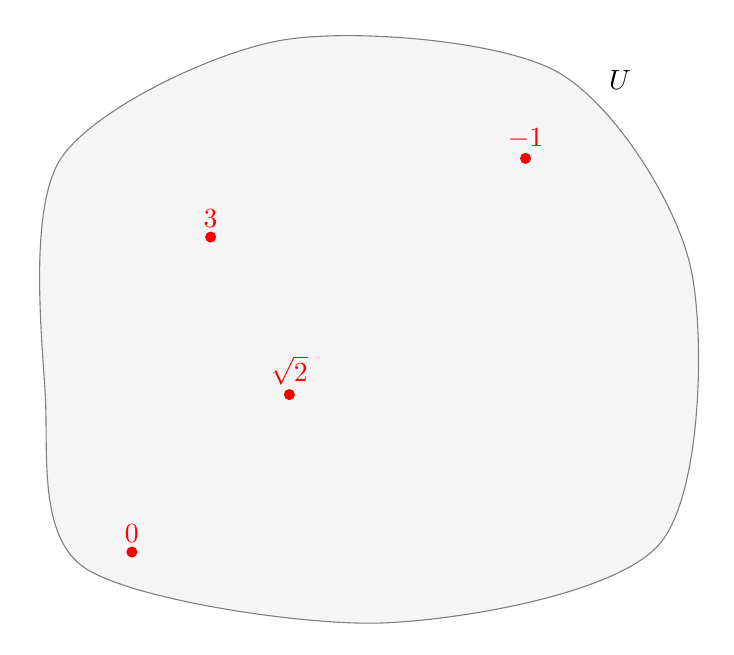
\begin{tikzpicture}
  \draw[gray,fill=gray!8] plot[smooth cycle] coordinates {(-3.6,-3.2)(0.2,-3.9)(3.7,-2.9)(4.1,0.6)(2.4,3.1)(-1.1,3.5)(-3.9,2)(-4.1,-1)}; \node at (3.2,3) {$U$};
  \fill[red] (-2,1) circle (2pt) node[above]{$3$};
  \fill[red] (-1,-1) circle (2pt) node[above]{$\sqrt2$};
  \fill[red] (2,2) circle (2pt) node[above]{$-1$};
  \fill[red] (-3,-3) circle (2pt) node[above]{$0$};
\end{tikzpicture}
\end{document}
